\documentclass[a4paper,sffamily,12pt]{article}

\usepackage[T1]{fontenc}
\usepackage[french]{babel}
\usepackage[utf8]{inputenc}

% Customization des listes
\usepackage{enumitem}
\usepackage{pifont}

% Insertion d'image
\usepackage{graphicx}

% Création de lien
\usepackage[colorlinks,linkcolor=blue]{hyperref}

% Formatage des titres de sections
\usepackage{titlesec}
\titleformat{\section}
  {\normalfont\Large\bfseries\sffamily}{\thesection.}{0.33em}{}[\hrule]
 
 % tableau rectangle 
%\usepackage{slashbox}
%\usepackage{tabularx}

 % En-tête
\usepackage{fancyhdr}
\pagestyle{fancy}
\renewcommand\headrulewidth{1pt}
\fancyhead[L]{Base de données 2}
\fancyhead[R]{$X6I0050$}

% Permet de mettre du texte au dessus du titre
\usepackage{titling}
\renewcommand{\maketitlehooka}{\noindent MAHIER Loïc \hfill groupe 601B \\ JEHANNO Clément \hfill \\ JAMET Félix \hfill \\ PHALAVANDISHVILI  Demetre}

% Titre
\title{\vspace{\fill}\LARGE\bfseries\sffamily Rapport préliminaire de projet\protect\footnote{rapport réalisé sous \LaTeX} \vspace{\fill}}

\begin{document}

	\date{} % Supprime la date
	\maketitle % Affiche le titre

	\thispagestyle{fancy} % Permet de mettre le titre sur la page ''fancy''
	
	\newpage
			
	\renewcommand{\contentsname}{Sommaire}
	\tableofcontents
	
	\newpage
	
	\section{Introduction}
		
		\vspace{0.5cm}
		
		Dans le cadre de ce projet nous devons créer une base de données. Nous avons décidé de modéliser la gestion de cinémas sur une grande échelle. Par exemple nous voulons savoir quels sont les cinémas de France, à qui ils appartiennent (Pathé,UGC, etc.) et ce qu'ils proposent. Comme notre modèle se base sur une certaine réalité, voici comment nous avons décomposé la chose, prenons  l'exemple d'un cinéma : \\
		\indent Le cinéma Pathé à Atlantis, dans la ville de Nantes. Tout d'abord on voit que un cinéma est identifié par une adresse et une ville. Ensuite, notre cinéma possède des salles dans lesquelles seront diffusés des films. Chaque film est composé d'une équipe d'acteurs, d'un réalisateur et d'une date de sortie. Il peut être compatible ou non avec la 3D. \\ 				
		\indent En ce qui concerne nos salles, elles possèdent un certain nombre de places qui sont réparties entre les places ''standards'', les places ''handicapés'' ainsi que les nouveaux sièges dBox (sièges bougeant en même temps que le film). Si elles sont compatibles, elles ont la possibilité de diffuser en 3D. \\
		\indent Une séance dans un cinéma donné correspond à une date de projection d'un certain film dans une salle spécifique à un horaire précis, le film étant diffusé ou non en 3D. Aujourd'hui si on va au cinéma il est possible de réserver sa séance, autrement dit, on réserve un certain nombre de places pour un film, à un horaire précis, dans un cinéma donné. 

		\vspace{0.5cm}
								
	\section{Répartition des tâches}

		\vspace{0.5cm}

		\noindent Voici comment nous nous sommes organisés pour répartir les tâches : \\
		\\
		\indent Tout d'abord après les premières semaines de cours nous nous sommes réunis pour décider ensemble d'un sujet. L'idée du cinéma est venue assez naturellement et nous paraissait être à la fois concrète et proche de la réalité.\\
		\indent Ensuite nous avons défini tous les attributs de notre table, en se demandant ensemble : Que voulons-nous faire ? Comment voulons nous le faire ? Un cinéma fonctionne t-il vraiment comme ça ? L'ajout de tel ou tel attribut est-il pertinent ? etc etc. Une fois nos attributs répartis nous avons chacun pris un cinéma (on en a 4) et chaque personne a remplit la partie du tableau qui correspondait à un cinéma. Après cela on a observé nos tuples sur tableur et on a relevé nos dépendances fonctionnelles.\\
		\indent Ensuite Demetre et Félix ont fait l'algorithme de décomposition et Loïc et Clément ont fait l'algorithme de Bernstein. On a mis en commun le résultat des deux algorithmes afin de voir si on avait la même chose ou non, et pourquoi. Pour finir, nous avons testé la normalisation de notre schéma avec l'outil mis à notre disposition en question 5.
						
		\vspace{0.5cm}
		
	\section{Table de base}	
		
		\vspace{0.5cm}
			
		Vous trouverez en annexe la table (\ref{table_p1}) contenant tous nos attributs ainsi que tous nos tuples. Celle-ci est en quatre parties à cause de sa taille conséquente.
		
		\vspace{0.5cm}						

	\section{Dépendances fonctionnelles}
	
		\vspace{0.5cm}
	
		A partir de la table ci-dessous contenant tous nos attributs, nous avons déduit les douze dépendances fonctionnelles ci-dessous. Pour ce faire nous avons ajouté des attributs (id) nous permettant de simplifier nos relations.\\
	
		\noindent- (1) idCine $\rightarrow$ adresse, ville \\
		- (2) adresse, ville $\rightarrow$ franchise, nbSalle \\
		- (3) idCine $\rightarrow$ franchise, nbSalles \\
		- (4) idCine, numSalle $\rightarrow$ salleCompatibleEn3D, nbPlaceStandard, nbPlaceHandicape,nbDbox \\
 		- (5) idFilm $\rightarrow$ nomFilm, dateSortie \\
		- (6) nomFilm, dateSortie $\rightarrow$ public, idReal, duree, compatible3D \\
		- (7) idFilm, role $\rightarrow$  idAct \\
		- (8) idReal $\rightarrow$ nomR, prenomR \\
		- (9) idAct $\rightarrow$ nomA, prenomA \\
		- (10) idClient $\rightarrow$ nomC, prenomC \\
		- (11) idClient, numReservation $\rightarrow$ nbPlaceStandardRes, nbPlaceHandicapeRes, nbPlaceDBoxRes, idSeance \\
		- (12) idSeance $\rightarrow$ idCine, horaire, dateProjection, numSalle, idFilm, diffusionEn3D \\
		
		\newpage
		
		Avec les dépendances fonctionnelles ci-dessus, nous obtenons le graphe des dépendances en annexe (\ref{graphe_dependances}). De cela nous déterminons la clé suivante : \{idCine, idClient, numReservation, role\}.
		
	\section{Algorithme de Bernstein}
	
		\vspace{0.5cm}

		\noindent L'algo de Bernstein se fait en 4 parties :
	
			\begin{enumerate}[label=\ding{228}]
				\item Calculer la CV(DF) et les clés. Si R est en 3FN on s'arrête. 
				\item Partitionner CV(DF) en groupe DFi (1 <= i <= k) tel que toutes les dfs d'un même groupe aient la même partie gauche. 
				\item Construire un schéma <Ri(Ui), DFi> pour chaque groupe DFi, où Ui est l'ensemble des attributs apparaissant dans DFi.
				\item Si aucun des schémas définis ne contient de clé X de R, rajouter un schéma <Rk+1(X), \{\}>.
			\end{enumerate}	
			
		\subsection{Calcul de CV(DF)}

			\vspace{0.5cm}

			\noindent La couverture minimale se fait en trois parties :

			\begin{enumerate}[label=\ding{228}]
				\item Toutes les dépendances doivent être élémentaires ; les décomposer si nécessaire.
				\item Eliminer les attributs superflus du coté gauche de la df.
				\item Eliminer les dfs redondantes.
			\end{enumerate}	
			
			\vspace{0.5cm}
				
			\subsubsection{Pas 1}

				\vspace{0.5cm}

				\noindent On décompose chacune des dfs en dfe : \\

				\noindent- (1) idCine $\rightarrow$ ville \\
				- (1) idCine $\rightarrow$ adresse \\
				- (2) adresse, ville $\rightarrow$ franchise \\
				- (2) adresse, ville $\rightarrow$ nbSalle \\
				- (3) idCine $\rightarrow$ franchise \\
				- (3) idCine $\rightarrow$ nbSalles \\
				- (4) idCine, numSalle $\rightarrow$ salleCompatibleEn3D \\
		 		- (4) idCine, numSalle $\rightarrow$ nbPlaceStandard \\
		 		- (4) idCine, numSalle $\rightarrow$ nbPlaceHandicape \\
		 		- (4) idCine, numSalle $\rightarrow$ nbDbox \\
		 		- (5) idFilm $\rightarrow$ nomFilm \\
		 		- (5) idFilm $\rightarrow$ dateSortie \\				 		
				- (6) nomFilm, dateSortie $\rightarrow$ public \\
				- (6) nomFilm, dateSortie $\rightarrow$ idReal \\
				- (6) nomFilm, dateSortie $\rightarrow$ duree \\
				- (6) nomFilm, dateSortie $\rightarrow$ compatible3D \\
				- (7) idFilm, role $\rightarrow$ idAct \\
				- (8) idReal $\rightarrow$ nomR \\
				- (8) idReal $\rightarrow$ prenomR \\						
				- (9) idAct $\rightarrow$ nomA \\
				- (9) idAct $\rightarrow$ prenomA \\						
				- (10) idClient $\rightarrow$ nomC \\
				- (10) idClient $\rightarrow$ prenomC \\						
				- (11) idClient, numReservation $\rightarrow$ idSeance \\
				- (11) idClient, numReservation $\rightarrow$ nbPlaceStandardRes \\
				- (11) idClient, numReservation $\rightarrow$ nbPlaceHandicapeRes \\
				- (11) idClient, numReservation $\rightarrow$ nbPlaceDBoxRes \\
				- (12) idSeance, idCine $\rightarrow$ horaire \\
				- (12) idSeance, idCine $\rightarrow$ dateProjection \\
				- (12) idSeance, idCine $\rightarrow$ numSalle \\
				- (12) idSeance, idCine $\rightarrow$ idFilm \\
				- (12) idSeance  idCine $\rightarrow$ diffusionEn3D \\
		
				\vspace{0.5cm}
									
			\subsubsection{Pas 2}

				\vspace{0.5cm}
	
				On prend toutes les dfs qui ont plus d'un attribut à gauche et on calcul leur fermeture. On élimine l'autre attribut si l'attribut de droite de la df apparaît dans le résultat, ou s'il apparaît dans le résultat de la fermeture. \\
				
				\noindent - (2) adresse, ville $\rightarrow$ franchise, nbSalle \\
					\\
					\underline{adresse+} \\
					adresse \\
					\underline{ville+} \\
					ville \\
				$\rightarrow$ Les deux attributs sont nécessaires. \\

				\noindent - (4) idCine, numSalle $\rightarrow$ salleCompatibleEn3D, nbPlaceStandard, nbPlaceHandicape,nbDbox \\
					\\
					\underline{idCine+} \\
					idCine / adresse / ville /franchise / nbSalle \\
					\underline{numSalle+} \\
					numSalle \\
				$\rightarrow$ Les deux attributs sont nécessaires. \\
				
				\noindent - (6) nomFilm, dateSortie $\rightarrow$ public, idReal, duree, compatible3D \\																						\\
					\underline{nomFilm+} \\
					nomFilm \\
					\underline{dateSortie+} \\
					dateSortie \\
				$\rightarrow$ Les deux attributs sont nécessaires. \\
			
				\noindent - (7) idFilm, role $\rightarrow$  idAct \\
					\\
					\underline{idFilm+} \\
					idFilm / nomFilm / dateSortie / public / idReal / duree / compatible3D / nomA / prenomA \\
					\underline{role+} \\
					role \\
				$\rightarrow$ Les deux attributs sont nécessaires. \\
					
				\noindent - (11) idClient, numReservation $\rightarrow$ nbPlaceStandardRes, nbPlaceHandicapeRes, nbPlaceDBoxRes, idSeance \\
					\\
					\underline{idClient+} \\
					idClient / nomC / prenomC \\
					\underline{numReservation+} \\
					numReservation \\	
				$\rightarrow$ Les deux attributs sont nécessaires. \\					
				
				\noindent - (12) idSeance, idCine $\rightarrow$ horaire, dateProjection, numSalle, idFilm, diffusionEn3D \\												
					\\
					\underline{idSeance+}\\
					idSeance \\
					\underline{idCine+}
					adresse / ville / franchise / nbSalle \\
				$\rightarrow$ Les deux attributs sont nécessaires. \\

				\vspace{0.5cm}

			\subsubsection{Pas 3}		
	
				\vspace{0.5cm}
	
				\noindent Eliminons tout d'abord les dfs qui sont préservées par transitivité : \\
	
					\noindent- (1) idCine $\rightarrow$ adresse, ville \\
					- (2) adresse, ville $\rightarrow$ franchise, nbSalle \\
					- (3) idCine $\rightarrow$ franchise, nbSalles \\
					
				Si l'on prend les dfs 1, 2 et 3, on remarque que l'on peut supprimer la 3 car on peut retrouver celle-ci par transitivité. Reprenons donc nos dfs restantes : \\
					
				\noindent- (1) idCine $\rightarrow$ adresse, ville \\
				- (2) adresse, ville $\rightarrow$ franchise, nbSalle \\
				- (3) idCine, numSalle $\rightarrow$ salleCompatibleEn3D, nbPlaceStandard, nbPlaceHandicape,nbDbox \\
		 		- (4) idFilm $\rightarrow$ nomFilm, dateSortie \\
				- (5) nomFilm, dateSortie $\rightarrow$ public, idReal, duree, compatible3D \\
				- (6) idFilm, role $\rightarrow$  idAct \\
				- (7) idReal $\rightarrow$ nomR, prenomR \\
				- (8) idAct $\rightarrow$ nomA, prenomA \\
				- (9) idClient $\rightarrow$ nomC, prenomC \\
				- (10) idClient, numReservation $\rightarrow$ nbPlaceStandardRes, nbPlaceHandicapeRes, nbPlaceDBoxRes, idSeance \\
				- (11) idSeance, idCine $\rightarrow$ horaire, dateProjection, numSalle, idFilm, diffusionEn3D \\
				
				\noindent A présent, analysons chaque dépendance fonctionelle une par une : \\
				
				\noindent - (1) idCine $\rightarrow$ adresse, ville \\
					\\
					\underline{idCine+} \\
					idCine\\									
				$\rightarrow$ La df est préservée. \\		
					
				\noindent - (2) adresse, ville $\rightarrow$ franchise, nbSalle \\
					\\
					\underline{adresse, ville+} \\
					adresse, ville \\									
				$\rightarrow$ La df est préservée. \\
				
				\noindent - (3) idCine, numSalle $\rightarrow$ salleCompatibleEn3D, nbPlaceStandard, nbPlaceHandicape,nbDbox \\
					\\
					\underline{idCine, numSalle+} \\
					idCine / adresse / ville / franchise / nbSalle / numSalle \\								
				$\rightarrow$ La df est préservée. \\													

				\noindent - (4) idFilm $\rightarrow$ nomFilm, dateSortie \\
					\\
					\underline{idFilm+} \\
					idFilm\\								
				$\rightarrow$ La df est préservée. \\	
				
				\noindent - (5) nomFilm, dateSortie $\rightarrow$ public, idReal, duree, compatible3D \\
					\\
					\underline{nomFilm, dateSortie+} \\
					nomFilm / dateSortie \\									
				$\rightarrow$ La df est préservée. \\	
				
				\noindent - (6) idFilm, role $\rightarrow$  idAct  \\
					\\
					\underline{idFilm, role+} \\
					idFilm / nomFilm / dateSortie / public / idReal / duree / compatible3D / nomR / prenomR / role \\					
				$\rightarrow$ La df est préservée. \\
																			
				\noindent - (7) idReal $\rightarrow$ nomP, prenomP \\
					\\
					\underline{idReal+} \\
					idReal \\								
				$\rightarrow$ La df est préservée. \\	
				
				\noindent - (8) idAct $\rightarrow$ nomP, prenomP \\
					\\
					\underline{idAct+} \\
					idAct \\									
				$\rightarrow$ La df est préservée. \\	

				\noindent - (9) idClient $\rightarrow$ nomC, prenomC \\
					\\
					\underline{idClient+} \\
					idClient \\									
				$\rightarrow$ La df est préservée. \\		

				\noindent - (10) idClient, numReservation $\rightarrow$ nbPlaceStandardRes, nbPlaceHandicapeRes, nbPlaceDBoxRes, idSeance \\
					\\
					\underline{idClient, numReservation+} \\
					idClient / nomC / prenomC / numReservation \\									
				$\rightarrow$ La df est préservée. \\		

				\noindent - (11) idSeance, idCine $\rightarrow$ horaire, dateProjection, numSalle, idFilm, diffusionEn3D \\
					\\
					\underline{idSeance, idCine+} \\
					idSeance / idCine / adresse / ville / franchise / nbSalle \\							
				$\rightarrow$ La df est préservée. \\							
				\\		
				
				\indent Ainsi, hormis la suppression d'une dépendance fonctionnelle transitive, nos dépendances fonctionelles ne changent pas. \\																
				\\
				\indent On constate que l'on est bien en 1FN, ainsi qu'en 2FN. Cependant nous ne sommes pas en 3FN. En effet, nous avons des attributs non clés, qui déterminent d'autres attributs non clés. Par exemple, adresse et ville sont deux attributs non clés qui déterminent franchise et nbSalle qui sont eux aussi non clés (df(2)). \\
				
				\vspace{0.5cm}
													
			\subsection{Partitionnement de la CV et construction des schémas} 	
			
				\vspace{0.5cm}
			
				\noindent R1 = \{\underline{idCine}, adresse, ville\} \\  DF1 = \{idCine $\rightarrow$ adresse, ville\} \\
				\\
				R2 = \{\underline{adresse, ville}, franchise, nbSalle\} \\ DF2 = \{adresse, ville $\rightarrow$ franchise, nbSalle\} \\
				\\
				R3 = \{\underline{idCine, numSalle}, salleCompatibleEn3D, nbPlaceStandard, nbPlaceHandicape, nbDbox\} \\ DF3 = \{idCine, numSalle, $\rightarrow$ salleCompatibleEn3D, nbPlaceStandard, nbPlaceHandicape, nbDbox\} \\
				\\
				R4 = \{\underline{idFilm}, nomFilm, dateSortie\} \\ DF4 = \{idFilm $\rightarrow$ nomFilm, dateSortie\} \\
				\\
				R5 = \{\underline{nomFilm, dateSortie}, public, idReal, duree, compatible3D\} \\ DF5 = \{nomFilm, dateSortie $\rightarrow$ public, idReal, duree, compatible3D\} \\	
				\\							
				R6 = \{\underline{idFilm, role}, idAct\} \\ DF6 = \{idFilm, role $\rightarrow$  idAct\} \\
				\\
				R7 = \{\underline{idReal}, nomR, prenomR\} \\ DF7 = \{idReal $\rightarrow$ nomR, prenomR\} \\
				\\
				R8 = \{\underline{idAct}, nomA, prenomA\} \\ DF8 = \{idAct $\rightarrow$ nomA, prenomA\} \\
				\\
				R9 = \{\underline{idClient}, nomC, prenomC\} \\ DF9 = \{idClient $\rightarrow$ nomC, prenomC\} \\ 
				\\
				R10 = \{\underline{idClient, numReservation}, nbPlaceStandardRes, nbPlaceHandicapeRes, nbPlaceDBoxRes, idSeance\} \\ DF10 = \{idClient, numReservation $\rightarrow$  nbPlaceStandardRes, nbPlaceHandicapeRes, nbPlaceDBoxRes, idSeance\} \\
				
				\newpage 
				
				R11 = \{\underline{idSeance, idCine}, horaire, dateProjection, numSalle, idFilm, diffusionEn3D\} \\ DF11 = \{idSeance, idCine $\rightarrow$ horaire, dateProjection, numSalle, idFilm, diffusionEn3D\} \\
				
				On constate que nous n'avons pas de relation contenant toutes nos clés, c'est pourquoi nous devons créer une relation pour cela, avec une dépendance fonctionnelle associée vide.\\
											
				\noindent R12 = \{\underline{idCine, idClient, numReservation, role}\} \\ DF12 = \{\} \\

				\vspace{0.5cm}

		\section{Algorithme de décomposition}

			\vspace{0.5cm}
			
			Nous avons pris tous nos attributs puis nous avons suivi l'algorithme de décomposition. C'est à dire que en fonction de nos attributs et de nos dépendances fonctionnelles, nous avons pris une dépendance et avons fait une relation en fonction de cette dépendance. Puis nous avons retiré nos attributs non clés du reste de la relation originale. Ensuite on a recommencé jusqu'à arriver à une partie ne contenant que des clés et plus de dépendance fonctionnelle.\\
			\indent On a commencé par les dépendances fonctionelles qui n'avaient qu'un attribut à gauche puis nous avons fini par celles qui avaient plusieurs attributs à gauche.

		\newpage
		
				\begin{figure}[!h]		
					\hspace{-2cm}
					{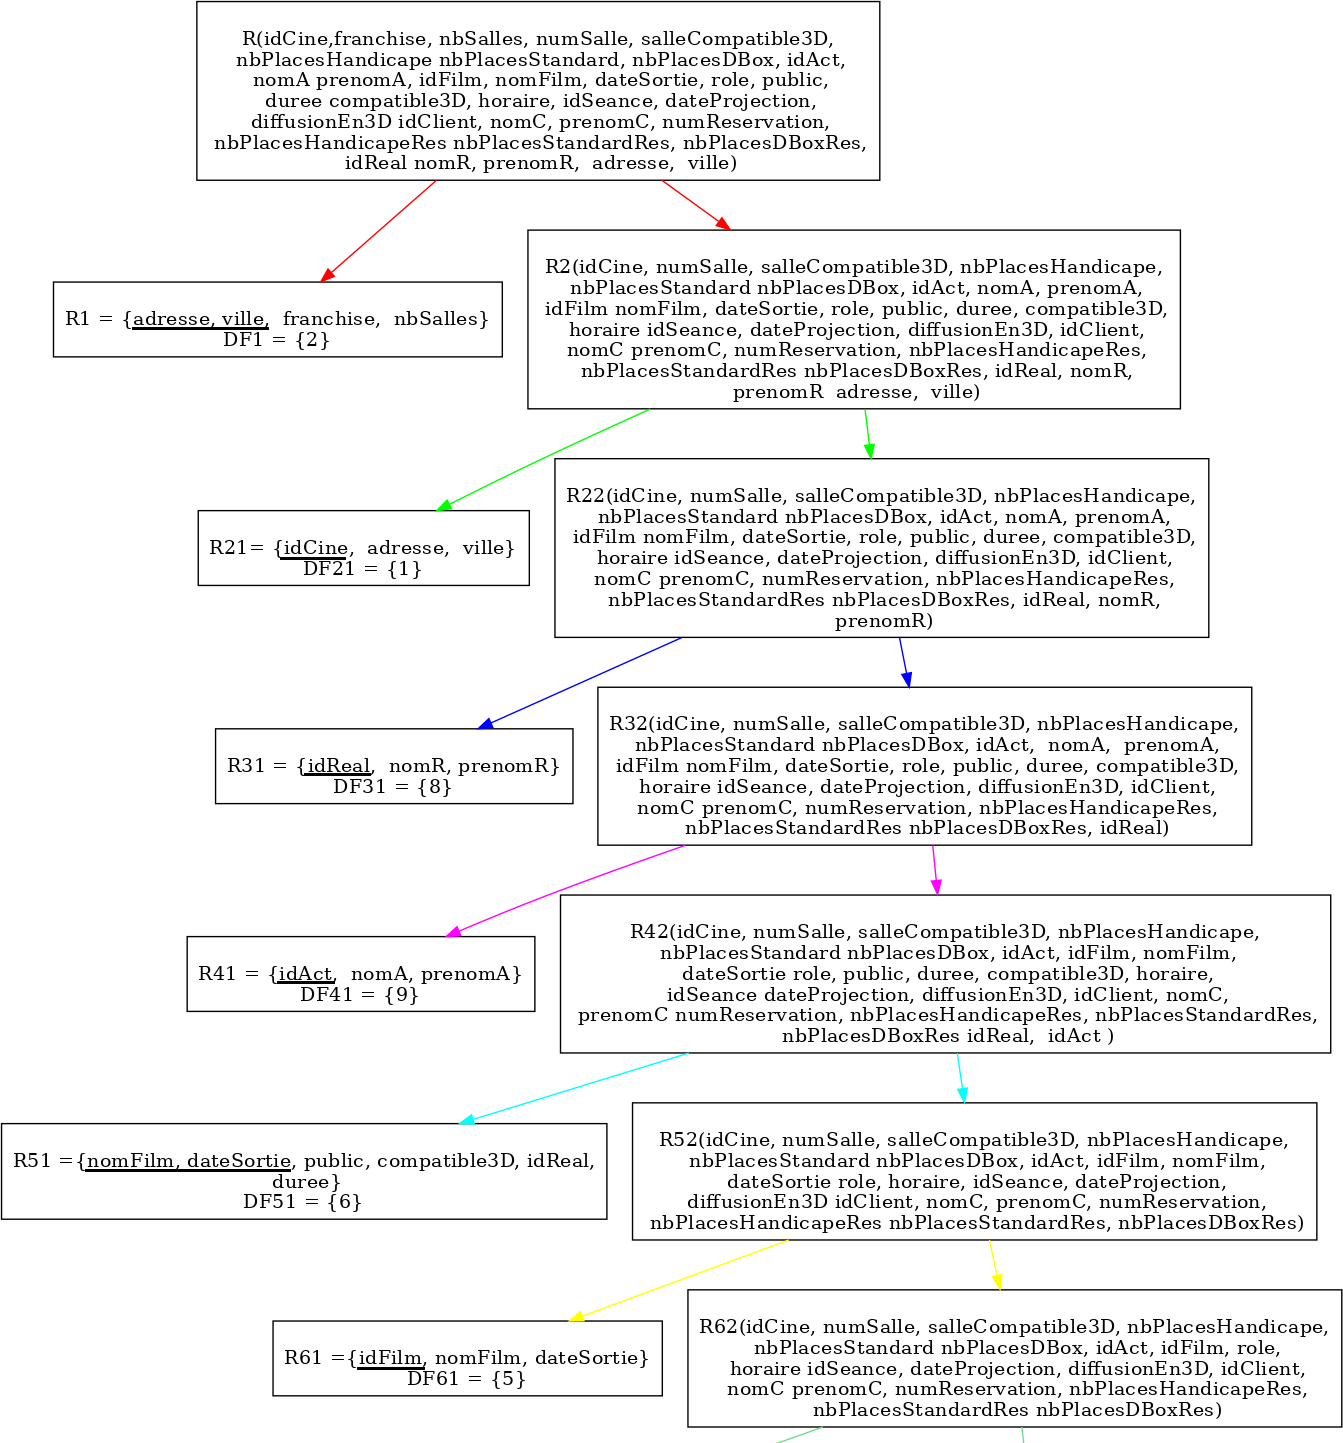
\includegraphics[height=19cm]{picture/decomp1.png}}
					\caption{Première partie de notre algorithme de décomposition}
					\label{decomp1}	
				\end{figure}	
			
				\begin{figure}[!h]		
					\hspace{-2cm}
					{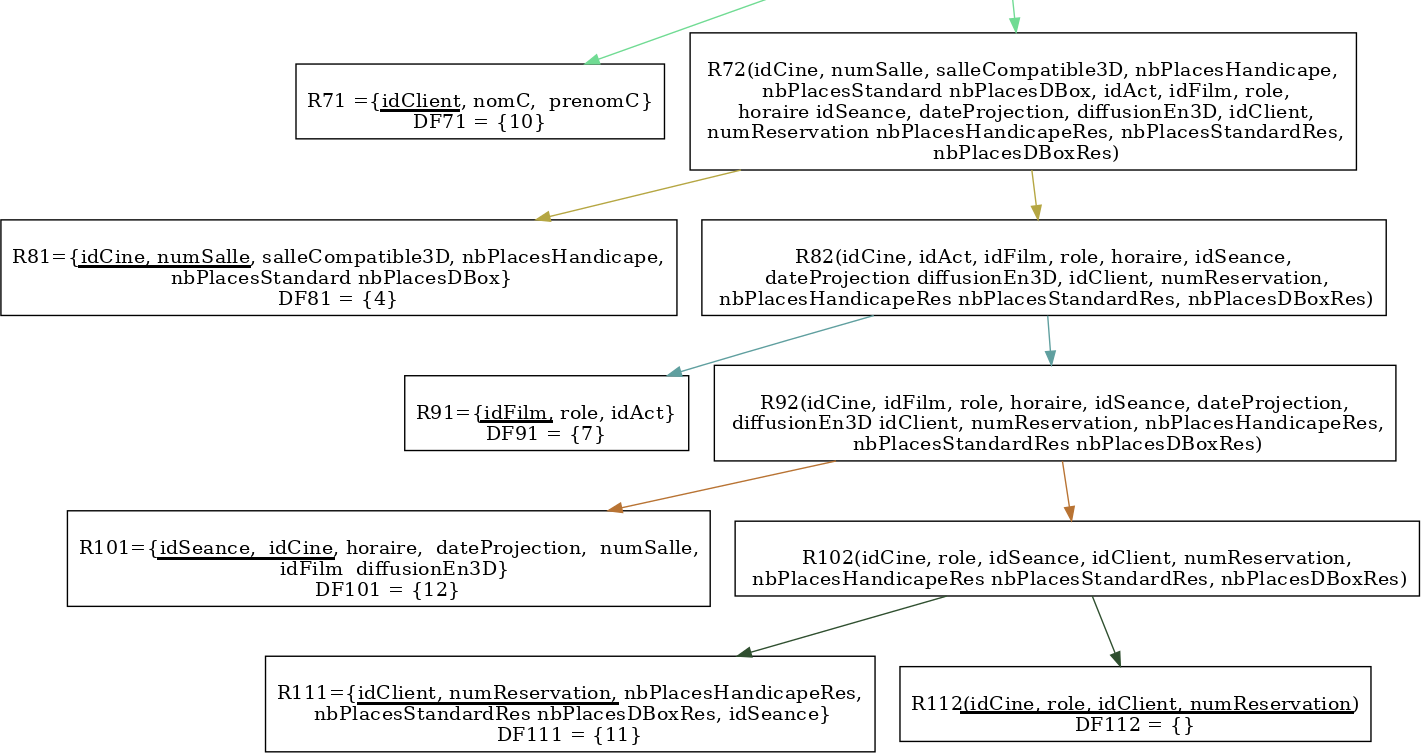
\includegraphics[height=9cm]{picture/decomp2.png}}
					\caption{Deuxième partie de notre algorithme de décomposition}
					\label{decomp2}	
				\end{figure}		

			\vspace{0.5cm}
		
		\section{Schéma de nos tables}

			\vspace{0.5cm}
					
		Pour le diagramme nous nous sommes basés sur le résultat de l'algorithme de décomposition qui nous a fourni des tables équivalentes aux 11 relations R1..R11. Cependant nous avons fusionné deux fois deux tables : la table R1 et R21 car cela nous paraît plus logique d'avoir pour chaque adresse, ville, franchise et nbSalles un seul idCine qui détermine un unique cinéma.\\
		\indent Cette table devient donc la table Cinema, ce qui donne plus de sens à notre modèle. Nous avons aussi fusionné R51 et R61 pour en faire une seule et même table Film pour les mêmes raisons.\\
		\indent Pour finir on a renommé toutes les autres tables pour leur donner un nom plus parlant : R31 est devenue Realisateur, R41 est devenue Acteur, R71 est devenue Client, R81 est devenue Salle, R91 est devenue Casting, R101 est devenue Seance et 111 est devenue Reservation.

				\begin{figure}[!h]		
					\hspace{-0.5cm}
					{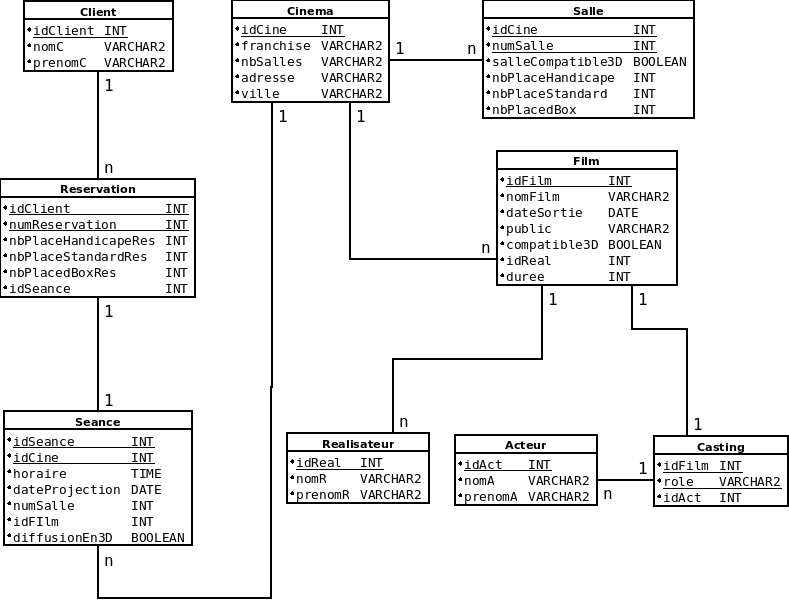
\includegraphics[height=12cm]{picture/DiagrammeUML.png}}
					\caption{Diagramme UML de nos tables}
					\label{UML}
					\vspace{0.5cm}	
				\end{figure}		


		\newpage

		\section{Conclusion préliminaire}

			\vspace{0.5cm}
			
			Cette première partie nous a permis de bien poser les bases de notre base de donnée. De plus, l'algorithme de décomposition nous permet d'obtenir des tables qui nous semblent cohérentes avec la réalité. Pour la suite, nous avons déjà quelques idées de contraintes, de triggers et de fonctions qu'il nous faudra intégrer pour bien gérer nos cinémas. \\			

			\newpage

			\section{Annexe}
							
				\begin{figure}[!h]		
					\centering
					\rotatebox{90}{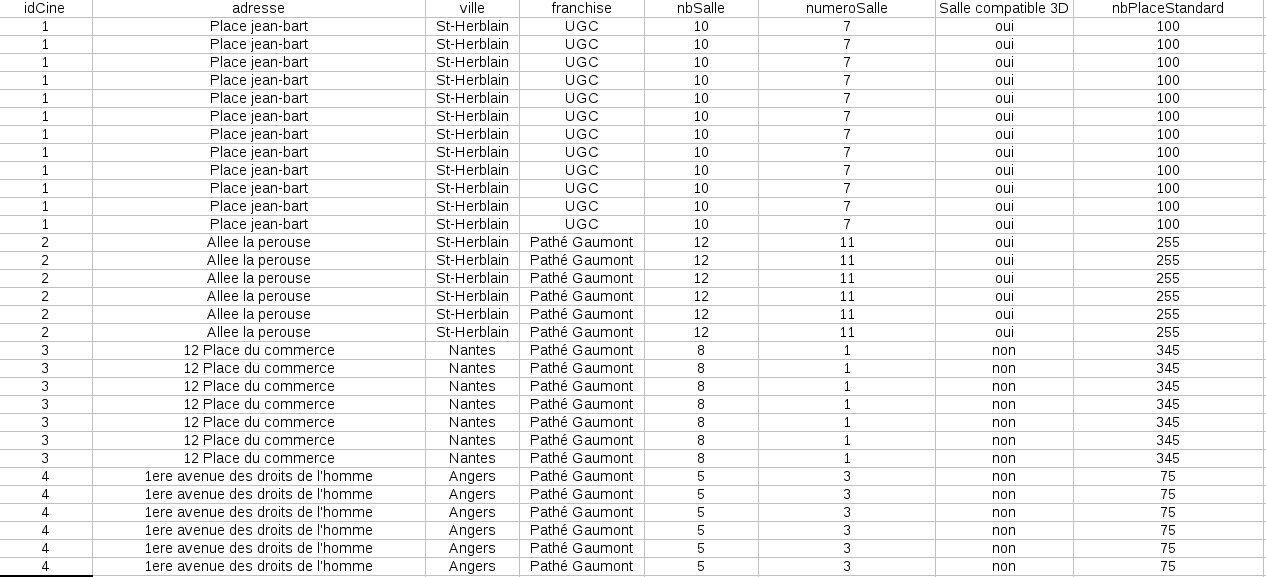
\includegraphics[height=8cm]{picture/table_p1_rogne.png}}
					\caption{Première partie de notre table contenant tous les attributs et quelques tuples}
					\label{table_p1}	
				\end{figure}			

				\begin{figure}[!h]
					\centering						
					\rotatebox{90}{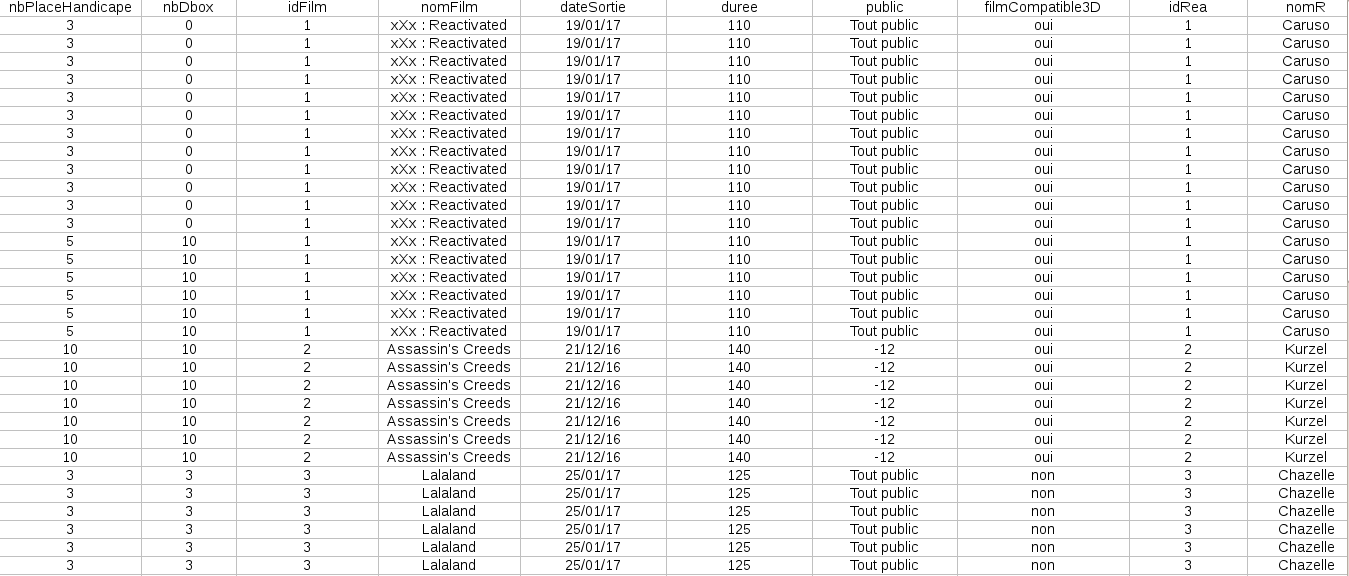
\includegraphics[height=8cm]{picture/table_p2_rogne.png}}
					\caption{Deuxième partie de notre table contenant tous les attributs et quelques tuples}
					\label{table_p2}	
				\end{figure}			

				\begin{figure}[!h]
					\centering						
					\rotatebox{90}{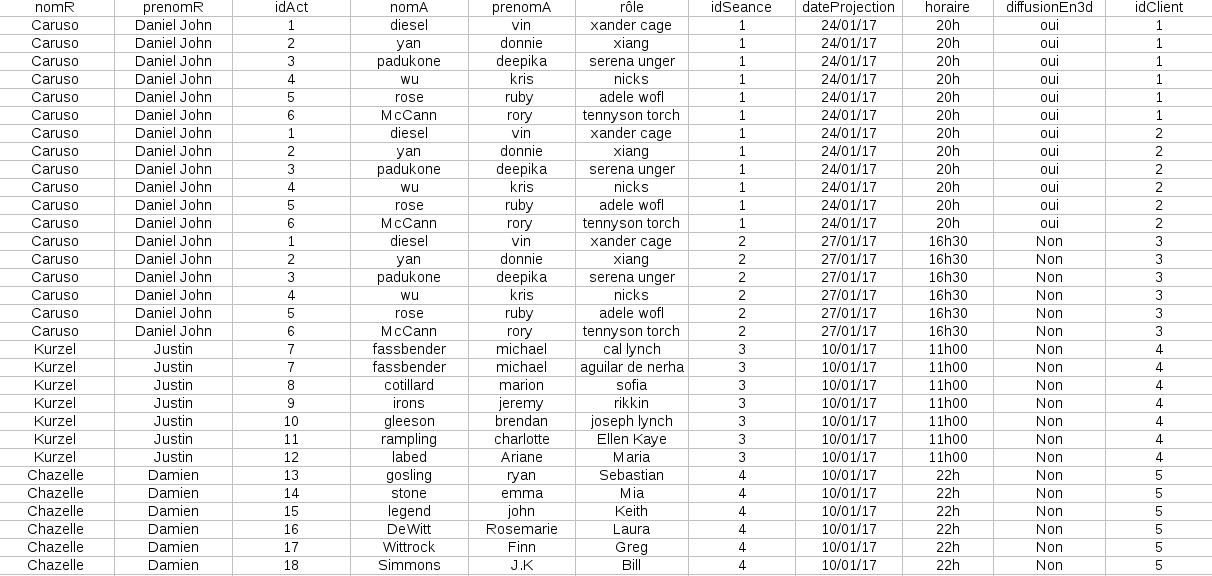
\includegraphics[height=9cm]{picture/table_p3_rogne.png}}
					\caption{Troisième partie de notre table contenant tous les attributs et quelques tuples}
					\label{table_p3}	
				\end{figure}	

				\begin{figure}[!h]
					\centering						
					\rotatebox{90}{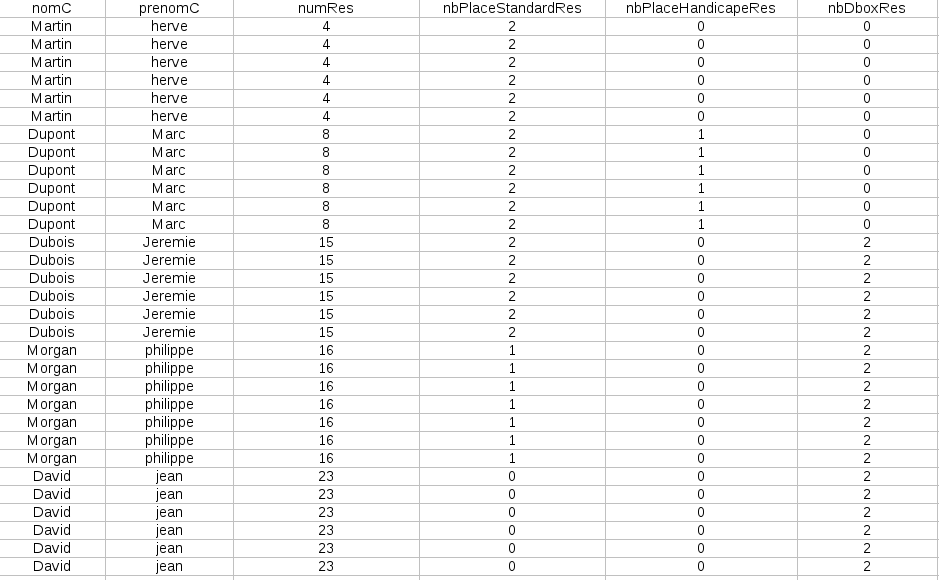
\includegraphics[height=10cm]{picture/table_p4_rogne.png}}
					\caption{Quatrième partie de notre table contenant tous les attributs et quelques tuples}
					\label{table_p4}	
				\end{figure}
				
				\begin{figure}[!h]
					\centering						
					\rotatebox{90}{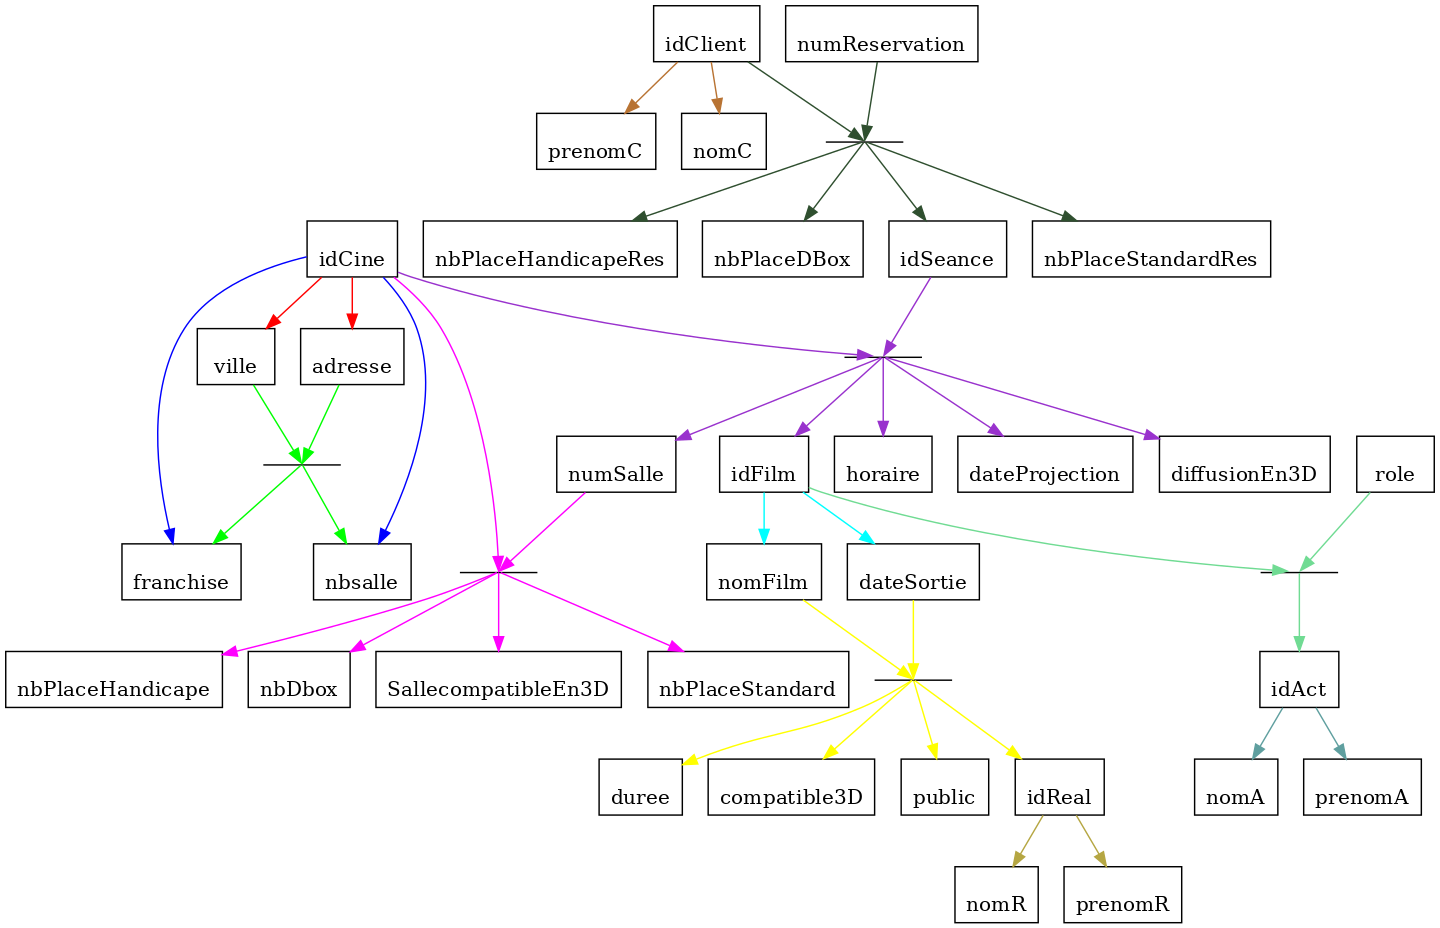
\includegraphics[height=12cm]{picture/graphe_dependances.png}}
					\caption{Graphe des dépendances}
					\label{graphe_dependances}	
				\end{figure}	
					
\end{document}
